%!TEX root = ../PRESENTATION_DGA.tex
\documentclass[11pt,class=book]{standalone}
%\usepackage[utf8]{inputenc}
\usepackage{fontenc}
\usepackage[table,svgnames]{xcolor}

\usepackage{pgf}
\usepackage{tikz}

\usepackage{array}
\usepackage{tabularx}
\usepackage{multirow}

\usetikzlibrary{shapes}
\usetikzlibrary{arrows.meta}
\usetikzlibrary{calc}

\definecolor{bg_color}{RGB}{250,250,229}

\colorlet{color1}{cyan!50}
\colorlet{color2}{red!30!green!40}
\colorlet{color3}{orange!50}
\colorlet{color4}{violet!60!blue!55}

\newganttlinktype{bartobardown}{
	\ganttsetstartanchor{south east}
	\ganttsetendanchor{north west}
	\draw [/pgfgantt/link] (\xLeft, \yUpper) -- (\xRight, \yLower);
}
\newganttlinktype{bartobarup}{
	\ganttsetstartanchor{north east}
	\ganttsetendanchor{south west}
	\draw [/pgfgantt/link] (\xLeft, \yUpper) -- (\xRight, \yLower);
}
\newganttlinktype{milestonetobardown}{
	\ganttsetstartanchor{south}
	\ganttsetendanchor{north west}
	\draw [/pgfgantt/link] (\xLeft, \yUpper) -- (\xRight, \yLower);
}
\newganttlinktype{bartomilestonedown}{
	\ganttsetstartanchor{south east}
	\ganttsetendanchor{north}
	\draw [/pgfgantt/link] (\xLeft, \yUpper) -- (\xRight, \yLower);
}


\begin{document}
	\begin{tikzpicture}[x=1pt,y=1pt,>=Latex]
		\tikzset{txt/.style={
			black,
			font=\footnotesize,
			text centered
		}}

		\node[
			anchor=south west,
			inner sep=0
		] (image) at (0,0)
		{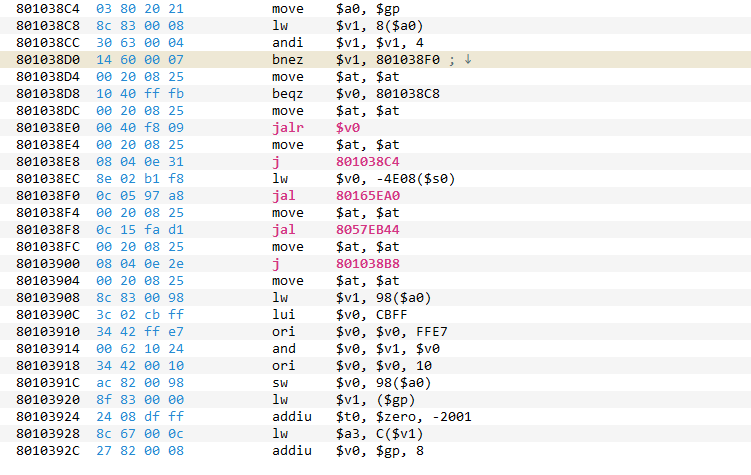
\includegraphics[width=0.9\textwidth]{GenDbg_GUI_Qt_Vue_code}};

		\begin{scope}[x={(image.south east)},y={(image.north west)}]
			%\draw[help lines,xstep=.1,ystep=.1] (0,0) grid (1,1);
			%\foreach \x in {0,1,...,9} { \node [anchor=north] at (\x/10,0) {\tiny 0.\x}; }
			%\foreach \y in {0,1,...,9} { \node [anchor=east] at (0,\y/10) {\tiny 0.\y}; }

			\pause
			%---------------------------------
			% Address
			\coordinate (addr1) at (0.02,1.01);
			\coordinate (addr2) at (0.11,1.01);
			\coordinate (addr) at ($(addr1)!0.5!(addr2)$);
			\draw (addr1) -- (addr2);
			\draw (addr1) -- ++(0,-0.01);
			\draw (addr2) -- ++(0,-0.01);
			\draw (addr) |- ++(-0.02,0.08) node[txt,anchor=east,text width=50] {Adresse de l'instruction};

			%---------------------------------
			% HEX value
			\coordinate (hex1) at (0.125,1.01);
			\coordinate (hex2) at (0.248,1.01);
			\coordinate (hex) at ($(hex1)!0.5!(hex2)$);
			\draw (hex1) -- (hex2);
			\draw (hex1) -- ++(0,-0.01);
			\draw (hex2) -- ++(0,-0.01);
			\draw (hex) -- ++(0,0.12) node[txt,anchor=south,text width=90] {Valeur hexadécimale de l'instruction};

			%---------------------------------
			% Instr
			\coordinate (instr1) at (0.36,1.01);
			\coordinate (instr2) at (0.54,1.01);
			\coordinate (instr) at ($(instr1)!0.5!(instr2)$);
			\draw (instr1) -- (instr2);
			\draw (instr1) -- ++(0,-0.01);
			\draw (instr2) -- ++(0,-0.01);
			\draw (instr) -- ++(0,0.05) node[txt,anchor=south] {Instruction désassemblée};

			\pause
			%---------------------------------
			% Current instr
			\coordinate (currentline) at (0.65,0.877);
			\draw[<-] (currentline) -- ++(0.1,0) node[txt,anchor=west,text width=90] {instruction courante (saut conditionnel)};

			\pause
			%---------------------------------
			% Jump direction
			\coordinate (jumpdir) at (0.6238,0.86);
			\draw[Bar-] (jumpdir) |- ++(0.1,-0.08) node[txt,anchor=west] {direction du saut};

			%---------------------------------
			% Non-conditional jump instr
			\coordinate (jump1) at (0.5,0.735);
			\coordinate (jump2) at (0.55,0.664);
			\coordinate (jump3) at (0.55,0.591);
			\coordinate (jump4) at (0.55,0.52);
			\coordinate (jump5) at (0.55,0.45);
			\coordinate (jumps) at ($(jump3)+(0.09,0)$);
			\draw[<-] (jump1) -| (jumps);
			\draw[<-] (jump2) -| (jumps);
			\draw[<-] (jump3) -| (jumps);
			\draw[<-] (jump4) -| (jumps);
			\draw[<-] (jump5) -| (jumps);
			\draw (jumps) -- ++(0.08,0) node[txt,anchor=west,text width=85] {instructions de saut non conditionnel};
		\end{scope}
	\end{tikzpicture}
\end{document}
